\documentclass{standalone}
\usepackage{tikz}
\usetikzlibrary{patterns, positioning}


\begin{document}
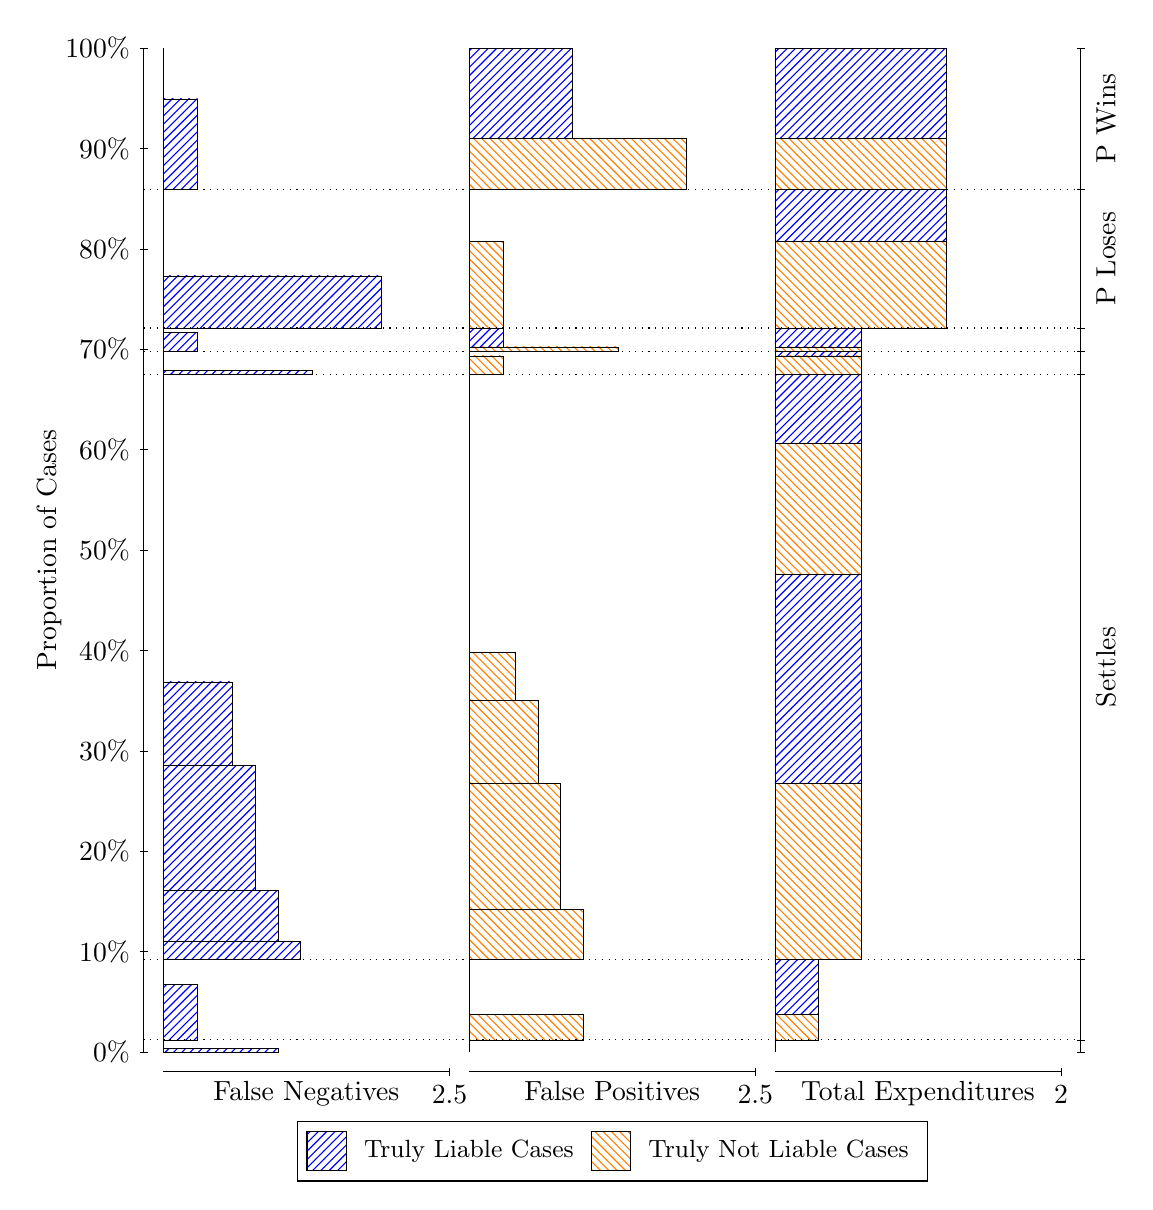
\begin{tikzpicture}
\draw[black, very thin] (1.5,1.75) -- (1.5,14.5);
\node[rotate=90, text=black, anchor=center] at (0.3, 8.125) {Proportion of Cases};
\draw[black, very thin] (1.45,1.75) -- (1.55,1.75);
\node[text=black, anchor=east] at (1.45, 1.75) {0\%};
\draw[black, very thin] (1.45,3.025) -- (1.55,3.025);
\node[text=black, anchor=east] at (1.45, 3.025) {10\%};
\draw[black, very thin] (1.45,4.3) -- (1.55,4.3);
\node[text=black, anchor=east] at (1.45, 4.3) {20\%};
\draw[black, very thin] (1.45,5.575) -- (1.55,5.575);
\node[text=black, anchor=east] at (1.45, 5.575) {30\%};
\draw[black, very thin] (1.45,6.85) -- (1.55,6.85);
\node[text=black, anchor=east] at (1.45, 6.85) {40\%};
\draw[black, very thin] (1.45,8.125) -- (1.55,8.125);
\node[text=black, anchor=east] at (1.45, 8.125) {50\%};
\draw[black, very thin] (1.45,9.4) -- (1.55,9.4);
\node[text=black, anchor=east] at (1.45, 9.4) {60\%};
\draw[black, very thin] (1.45,10.675) -- (1.55,10.675);
\node[text=black, anchor=east] at (1.45, 10.675) {70\%};
\draw[black, very thin] (1.45,11.95) -- (1.55,11.95);
\node[text=black, anchor=east] at (1.45, 11.95) {80\%};
\draw[black, very thin] (1.45,13.225) -- (1.55,13.225);
\node[text=black, anchor=east] at (1.45, 13.225) {90\%};
\draw[black, very thin] (1.45,14.5) -- (1.55,14.5);
\node[text=black, anchor=east] at (1.45, 14.5) {100\%};

\draw[black, very thin] (13.4,1.75) -- (13.4,14.5);
\draw[black, very thin] (13.35,1.75) -- (13.45,1.75);
\node[anchor=west] at (13.35, 1.75) {};
\draw[black, very thin] (13.35,1.9046) -- (13.45,1.9046);
\node[anchor=west] at (13.35, 1.9046) {};
\draw[black, very thin] (13.35,2.9252) -- (13.45,2.9252);
\node[anchor=west] at (13.35, 2.9252) {};
\draw[black, very thin] (13.35,10.351) -- (13.45,10.351);
\node[anchor=west] at (13.35, 10.351) {};
\draw[black, very thin] (13.35,10.647) -- (13.45,10.647);
\node[anchor=west] at (13.35, 10.647) {};
\draw[black, very thin] (13.35,10.944) -- (13.45,10.944);
\node[anchor=west] at (13.35, 10.944) {};
\draw[black, very thin] (13.35,12.706) -- (13.45,12.706);
\node[anchor=west] at (13.35, 12.706) {};
\draw[black, very thin] (13.35,14.5) -- (13.45,14.5);
\node[anchor=west] at (13.35, 14.5) {};

\draw[black, very thin, pattern color=blue, pattern=north east lines] (1.75,1.75) rectangle (3.2033,1.7924);
\draw[black, very thin, pattern color=orange, pattern=north west lines] (1.75,1.7924) rectangle (1.75,1.9046);
\draw[black, very thin, pattern color=blue, pattern=north east lines] (1.75,1.9046) rectangle (2.186,2.6058);
\draw[black, very thin, pattern color=orange, pattern=north west lines] (1.75,2.6058) rectangle (1.75,2.9252);
\draw[black, very thin, pattern color=blue, pattern=north east lines] (1.75,2.9252) rectangle (3.494,3.1585);
\draw[black, very thin, pattern color=blue, pattern=north east lines] (1.75,3.1585) rectangle (3.2033,3.7976);
\draw[black, very thin, pattern color=blue, pattern=north east lines] (1.75,3.7976) rectangle (2.9127,5.3914);
\draw[black, very thin, pattern color=blue, pattern=north east lines] (1.75,5.3914) rectangle (2.622,6.4509);
\draw[black, very thin, pattern color=orange, pattern=north west lines] (1.75,6.4509) rectangle (1.75,10.351);
\draw[black, very thin, pattern color=blue, pattern=north east lines] (1.75,10.351) rectangle (3.6393,10.409);
\draw[black, very thin, pattern color=orange, pattern=north west lines] (1.75,10.409) rectangle (1.75,10.647);
\draw[black, very thin, pattern color=blue, pattern=north east lines] (1.75,10.647) rectangle (2.186,10.886);
\draw[black, very thin, pattern color=orange, pattern=north west lines] (1.75,10.886) rectangle (1.75,10.944);
\draw[black, very thin, pattern color=blue, pattern=north east lines] (1.75,10.944) rectangle (4.5113,11.605);
\draw[black, very thin, pattern color=orange, pattern=north west lines] (1.75,11.605) rectangle (1.75,12.706);
\draw[black, very thin, pattern color=blue, pattern=north east lines] (1.75,12.706) rectangle (2.186,13.854);
\draw[black, very thin, pattern color=orange, pattern=north west lines] (1.75,13.854) rectangle (1.75,14.5);
\draw[black, very thin, pattern color=orange, pattern=north west lines] (5.6333,1.75) rectangle (5.6333,1.8622);
\draw[black, very thin, pattern color=blue, pattern=north east lines] (5.6333,1.8622) rectangle (5.6333,1.9046);
\draw[black, very thin, pattern color=orange, pattern=north west lines] (5.6333,1.9046) rectangle (7.0867,2.224);
\draw[black, very thin, pattern color=blue, pattern=north east lines] (5.6333,2.224) rectangle (5.6333,2.9252);
\draw[black, very thin, pattern color=orange, pattern=north west lines] (5.6333,2.9252) rectangle (7.0867,3.5643);
\draw[black, very thin, pattern color=orange, pattern=north west lines] (5.6333,3.5643) rectangle (6.796,5.1581);
\draw[black, very thin, pattern color=orange, pattern=north west lines] (5.6333,5.1581) rectangle (6.5053,6.2176);
\draw[black, very thin, pattern color=orange, pattern=north west lines] (5.6333,6.2176) rectangle (6.2147,6.8255);
\draw[black, very thin, pattern color=blue, pattern=north east lines] (5.6333,6.8255) rectangle (5.6333,10.351);
\draw[black, very thin, pattern color=orange, pattern=north west lines] (5.6333,10.351) rectangle (6.0693,10.589);
\draw[black, very thin, pattern color=blue, pattern=north east lines] (5.6333,10.589) rectangle (5.6333,10.647);
\draw[black, very thin, pattern color=orange, pattern=north west lines] (5.6333,10.647) rectangle (7.5227,10.705);
\draw[black, very thin, pattern color=blue, pattern=north east lines] (5.6333,10.705) rectangle (6.0693,10.944);
\draw[black, very thin, pattern color=orange, pattern=north west lines] (5.6333,10.944) rectangle (6.0693,12.044);
\draw[black, very thin, pattern color=blue, pattern=north east lines] (5.6333,12.044) rectangle (5.6333,12.706);
\draw[black, very thin, pattern color=orange, pattern=north west lines] (5.6333,12.706) rectangle (8.3947,13.352);
\draw[black, very thin, pattern color=blue, pattern=north east lines] (5.6333,13.352) rectangle (6.9413,14.5);
\draw[black, very thin, pattern color=orange, pattern=north west lines] (9.5167,1.75) rectangle (9.5167,1.8622);
\draw[black, very thin, pattern color=blue, pattern=north east lines] (9.5167,1.8622) rectangle (9.5167,1.9046);
\draw[black, very thin, pattern color=orange, pattern=north west lines] (9.5167,1.9046) rectangle (10.062,2.224);
\draw[black, very thin, pattern color=blue, pattern=north east lines] (9.5167,2.224) rectangle (10.062,2.9252);
\draw[black, very thin, pattern color=orange, pattern=north west lines] (9.5167,2.9252) rectangle (10.607,5.1581);
\draw[black, very thin, pattern color=blue, pattern=north east lines] (9.5167,5.1581) rectangle (10.607,7.8114);
\draw[black, very thin, pattern color=orange, pattern=north west lines] (9.5167,7.8114) rectangle (10.607,9.4789);
\draw[black, very thin, pattern color=blue, pattern=north east lines] (9.5167,9.4789) rectangle (10.607,10.351);
\draw[black, very thin, pattern color=orange, pattern=north west lines] (9.5167,10.351) rectangle (10.607,10.589);
\draw[black, very thin, pattern color=blue, pattern=north east lines] (9.5167,10.589) rectangle (10.607,10.647);
\draw[black, very thin, pattern color=orange, pattern=north west lines] (9.5167,10.647) rectangle (10.607,10.705);
\draw[black, very thin, pattern color=blue, pattern=north east lines] (9.5167,10.705) rectangle (10.607,10.944);
\draw[black, very thin, pattern color=orange, pattern=north west lines] (9.5167,10.944) rectangle (11.697,12.044);
\draw[black, very thin, pattern color=blue, pattern=north east lines] (9.5167,12.044) rectangle (11.697,12.706);
\draw[black, very thin, pattern color=orange, pattern=north west lines] (9.5167,12.706) rectangle (11.697,13.352);
\draw[black, very thin, pattern color=blue, pattern=north east lines] (9.5167,13.352) rectangle (11.697,14.5);
\draw[black, dotted] (1.5,1.9046) -- (13.4,1.9046);
\draw[black, dotted] (1.5,2.9252) -- (13.4,2.9252);
\draw[black, dotted] (1.5,10.351) -- (13.4,10.351);
\draw[black, dotted] (1.5,10.647) -- (13.4,10.647);
\draw[black, dotted] (1.5,10.944) -- (13.4,10.944);
\draw[black, dotted] (1.5,12.706) -- (13.4,12.706);
\draw[black, very thin] (1.75,1.5) -- (5.3833,1.5);
\node[text=black, anchor=north] at (3.5667, 1.5) {False Negatives};
\draw[black, very thin] (5.3833,1.45) -- (5.3833,1.55);
\node[text=black, anchor=north] at (5.3833, 1.45) {2.5};

\draw[black, very thin] (5.6333,1.5) -- (9.2667,1.5);
\node[text=black, anchor=north] at (7.45, 1.5) {False Positives};
\draw[black, very thin] (9.2667,1.45) -- (9.2667,1.55);
\node[text=black, anchor=north] at (9.2667, 1.45) {2.5};

\draw[black, very thin] (9.5167,1.5) -- (13.15,1.5);
\node[text=black, anchor=north] at (11.333, 1.5) {Total Expenditures};
\draw[black, very thin] (13.15,1.45) -- (13.15,1.55);
\node[text=black, anchor=north] at (13.15, 1.45) {2};



\node[text=black, centered, rotate=90] at (13.72, 6.6382) {Settles};


\node[text=black, centered, rotate=90] at (13.72, 11.825) {P Loses};
\node[text=black, centered, rotate=90] at (13.72, 13.603) {P Wins};

\draw (7.449999999999999,1.5) node[draw=none] (baseCoordinate) {};
\begin{scope}[align=center]
        \matrix[scale=0.5, draw=black, below=0.5cm of baseCoordinate, nodes={draw}, column sep=0.1cm]{
            \node[rectangle, draw, minimum width=0.5cm, minimum height=0.5cm, pattern color=blue, pattern=north east lines] {}; &
            \node[draw=none, font=\small, text=black] (B) {Truly Liable Cases}; &
            \node[rectangle, draw, minimum width=0.5cm, minimum height=0.5cm, pattern color=orange, pattern=north west lines] {}; &
            \node[draw=none, font=\small, text=black] (B) {Truly Not Liable Cases}; \\
            };
\end{scope}

\end{tikzpicture}
\end{document}